\documentclass[fleqn]{article}
\usepackage[nodisplayskipstretch]{setspace}
\usepackage{amsmath, nccmath, bm}
\usepackage{amssymb}
\usepackage{enumitem}
\usepackage{graphicx}
\usepackage{float}

\newcommand{\zerodisplayskip}{
	\setlength{\abovedisplayskip}{0pt}%
	\setlength{\belowdisplayskip}{0pt}%
	\setlength{\abovedisplayshortskip}{0pt}%
	\setlength{\belowdisplayshortskip}{0pt}%
	\setlength{\mathindent}{0pt}}
	
\newcommand{\norm}[1]{\left \lVert #1 \right \rVert}

\makeatletter
	\newenvironment{equationCenter}{\@fleqnfalse\begin{equation*}}{\end{equation*}}
\makeatother

\title{Exam 2}
\author{Owen Sowatzke}
\date{November 12, 2024}

\begin{document}

	\offinterlineskip
	\setlength{\lineskip}{12pt}
	\zerodisplayskip
	\maketitle
	
	\begin{enumerate}
		\item A four-dimensional (4-D) signal constellation is described by the following set of points $\{\pm a, \pm a, \pm a, \pm a\}$ ($a>0$). Different signal constellation points are used with the same probability. Determine the average symbol energy. Chose the appropriate basis functions $\{\Phi_1(t), \Phi_2(t), \Phi_3(t), \Phi_4(t)\}$ and express the signal constellation points in terms of basis functions. For AWGN channel, determine the average symbol error probability as a function of the average energy ($E_{av}$). Evaluate now the average symbol error probability in the presence of Rayleigh fading. Finally, evaluate the symbol error probability in the presence of Rayleigh fading when \underline{maximum-ratio combining diversity} is used. \underline{Note}: Do not evaluate integrals.

		Average symbol energy:
		
		\begin{equation*}
			E_{av} = \frac{1}{16}\sum_{i=0}^{16}{E_i} = \frac{1}{16}\sum_{i=0}^{16}{\norm{s_i}^2} = \frac{1}{16}\sum_{i}^{16}{4a^2} = 4a^2
		\end{equation*}
		
		Define the basis functions as follows:
		
		\begin{equation*}
			\Phi_k(t) = \sqrt{\frac{2}{T}}\cos\left(\frac{2{\pi}kt}{T}\right),\quad 0 \leq t < T
		\end{equation*}
		
		We can prove the basis functions form an orthonormal basis:
		
		\begin{equation*}
			\int_{0}^{T}{\Phi_j(t)\Phi_k^*(t)dt} = \frac{2}{T}\int_{0}^{T}{\cos\left(\frac{2{\pi}jt}{T}\right)\cos\left(\frac{2{\pi}kt}{T}\right)dt}
		\end{equation*}
		
		\begin{equation*}
			= \frac{1}{T}\int_{0}^{T}{\cos\left(\frac{2{\pi}(j+k)t}{T}\right)dt} + \frac{1}{T}\int_{0}^{T}{\cos\left(\frac{2{\pi}(j-k)t}{T}\right)dt}
		\end{equation*}
		
		\begin{equation*}
			= \begin{cases}
				1 & j = k \\
				0 & j \neq k
			\end{cases}
		\end{equation*}
		
		$\therefore$ $\Phi_k(t)$ forms an orthonormal basis.
		
		The constellations points can be expressed in terms of the basis functions as follows:
		
		\begin{equation*}
			s_m(t) = \sum_{k=0}^{3}{a\cos({\pi}n_{mk})\cos\left(\frac{2{\pi}kt}{T}\right)}
		\end{equation*}
		
		where $\{0 \leq n_{mk} \leq 1\ \vert\ n_{mk} \in Z\}$
		
		\begin{equation*}
			\Rightarrow s_m(t) = \sum_{k=0}^{3}{a\cos\left(\frac{2{\pi}kt}{T}+{\pi}n_{mk}\right)}
		\end{equation*}
		
		We define $n_{mk}$ as follows for each element of $\mathbf{s_m}$
		
		\begin{equation*}
			n_{mk} = \begin{cases}
				0 & s_{mk} \geq 0\\
				1 & s_{mk} < 0
			\end{cases}
		\end{equation*}
		
		The symbol error probability $P_s(\rho)$ can be approximated as follows:
		
		\begin{equation*}
			P_s(\rho) \approx M_{d_\text{min}}Q\left(\frac{d_\text{min}}{\sqrt{2N_0}}\right)
		\end{equation*}
		
		where $M_{d_\text{min}}$ is the number of nearest neighbors and $d_\text{min}$ is the minimum distance between neighboring constellation points.
		
		For each point in the constellation, there will be $M_{d_\text{min}} = 4$ nearest neighbors (one element different and all others the same). For each nearest neighbor, $d_\text{min} = 2a$.
		
		\begin{equation*}
			\Rightarrow P_s(\rho) \approx 4Q\left(\frac{2a}{\sqrt{2N_0}}\right) = 4Q\left(\sqrt{\frac{E_{av}}{2N_0}}\right)= 4Q\left(\sqrt{\frac{\rho}{2}}\right)
		\end{equation*}
		
		In Rayleigh fading, the average probability of symbol error is given as follows:
		
		\begin{equation*}
			\bar{P}_s = \int_{0}^{\infty}{P_s(\rho)f(\rho)d\rho} = \int_{0}^{\infty}{4Q\left(\sqrt{\frac{\rho}{2}}\right)\frac{1}{\bar{\rho}}e^{-\frac{\rho}{\bar{\rho}}}d\rho}
		\end{equation*}
		
		When Maximum-Ratio Combining is Used:
		
		\begin{equation*}
			\bar{P}_s = \int_{0}^{\infty}{P_s(\rho)f_{\rho_{\oplus}}(\rho)d\rho} = \int_{0}^{\infty}{P_s(\rho)\frac{\rho^{M-1}e^{-\rho/\bar{\rho}}}{\bar{\rho}^M(M-1)!}d\rho}
		\end{equation*}
		
		\begin{equation*}
			= \int_{0}^{\infty}{4Q\left(\sqrt{\frac{\rho}{2}}\right)\frac{\rho^{M-1}e^{-\rho/\bar{\rho}}}{\bar{\rho}^M(M-1)!}d\rho}
		\end{equation*}
		
		\item In this problem, we study the receiver diversity based on equal gain combining (EGC). Let us assume that either BPSK or QPSK is used to transmit messages over a generalized-fading wireless channel. According to
the generalized-fading channel model, the signal envelope at the ith receiver branch ($i=1,2,\ldots,L$) follows $\alpha$-$\mu$ distribution with probability density function (PDF) given by

		\begin{equationCenter}
			f_{R_i}(r_i) = \frac{\alpha_i\mu_i^{\mu_i}r_i^{\alpha_i\mu_i-1}}{\hat{r}_i^{\alpha_i\mu_i}\Gamma(\mu_i)}\text{exp}\left(\mu_i\frac{r_i^{\alpha_i}}{\hat{r}_i^{\alpha_i}}\right),
		\end{equationCenter}
		
		where $\alpha_i > 0$ is the parameter of nonlinearity, $\Gamma(.)$ is the Gamma function, and $\mu_i > 0$ is the inverse of the normalized variance of $r_i^{\alpha_i}$, namely $\mu_i = \text{E}^2\left\{r_i^{\alpha_i}\right\}/\text{Var}\left\{r_i^{\alpha_i}\right\}$, where $\text{E}\{x\}$ is the expectation operator, and $\hat{r}_i$ is a $\alpha_i$-root mean value $\hat{r}_i=\sqrt[\alpha_i]{\text{E}\left\{r_i^{\alpha_i}\right\}}$. If the phase estimation is done from unmodulated carrier by using phase-locked loop (PLL) and if only the Gaussian noise is present in the phase-locked loop circuit, then the PDF of this phase error is

		\begin{equationCenter}
			p_{\varphi_i}(\varphi_i) = \frac{1}{2\pi}\frac{\text{exp}(\zeta_i\text{cos}(\varphi_i))}{I_0(\zeta_i)}, \quad -\pi < \varphi_i \leq \pi,
		\end{equationCenter}
		
		where $I_0(x)$ is the modified Bessel function of the first kind and zero order for the argument x, $\zeta_i$ is the SNR in the PLL circuit in the i-th receiver branch. Write the expressions for the average bit error probability of uncoded BPSK and QPSK signal detections in the presence of phase error and $\alpha$-$\mu$ fading assuming that EGC receiver is used. \underline{Note}: Do not evaluate the integrals.
		
		The signal in each of the receiver branches can be written as:
		
		\begin{equation*}
			s_i(t) = r_i(t)e^{j(\omega_ct + \phi(t) + \gamma_i(t))} + n_i(t)
		\end{equation*}
		
		where $r_i(t)$ is the signal envelope in the i-th branch, $\omega_c$ is the carrier frequency, $\phi(t)$ is the phase of the transmitted symbols (common to all branches), $\gamma_i(t)$ is the phase error of the i-th branch, and $n_i(t)$ is the noise on the i-th branch.
		
		In equal gain combining, co-phasing is performed to account for the phase error between branches. This is equivalent to mixing each signal with $e^{-j(\omega_ct + \hat{\gamma}_i(t))}$ where $\hat{\gamma}_i(t)$ is an estimate of the phase error on the i-th receiver branch.
		
		\begin{figure}[H]
			\centerline{\fbox{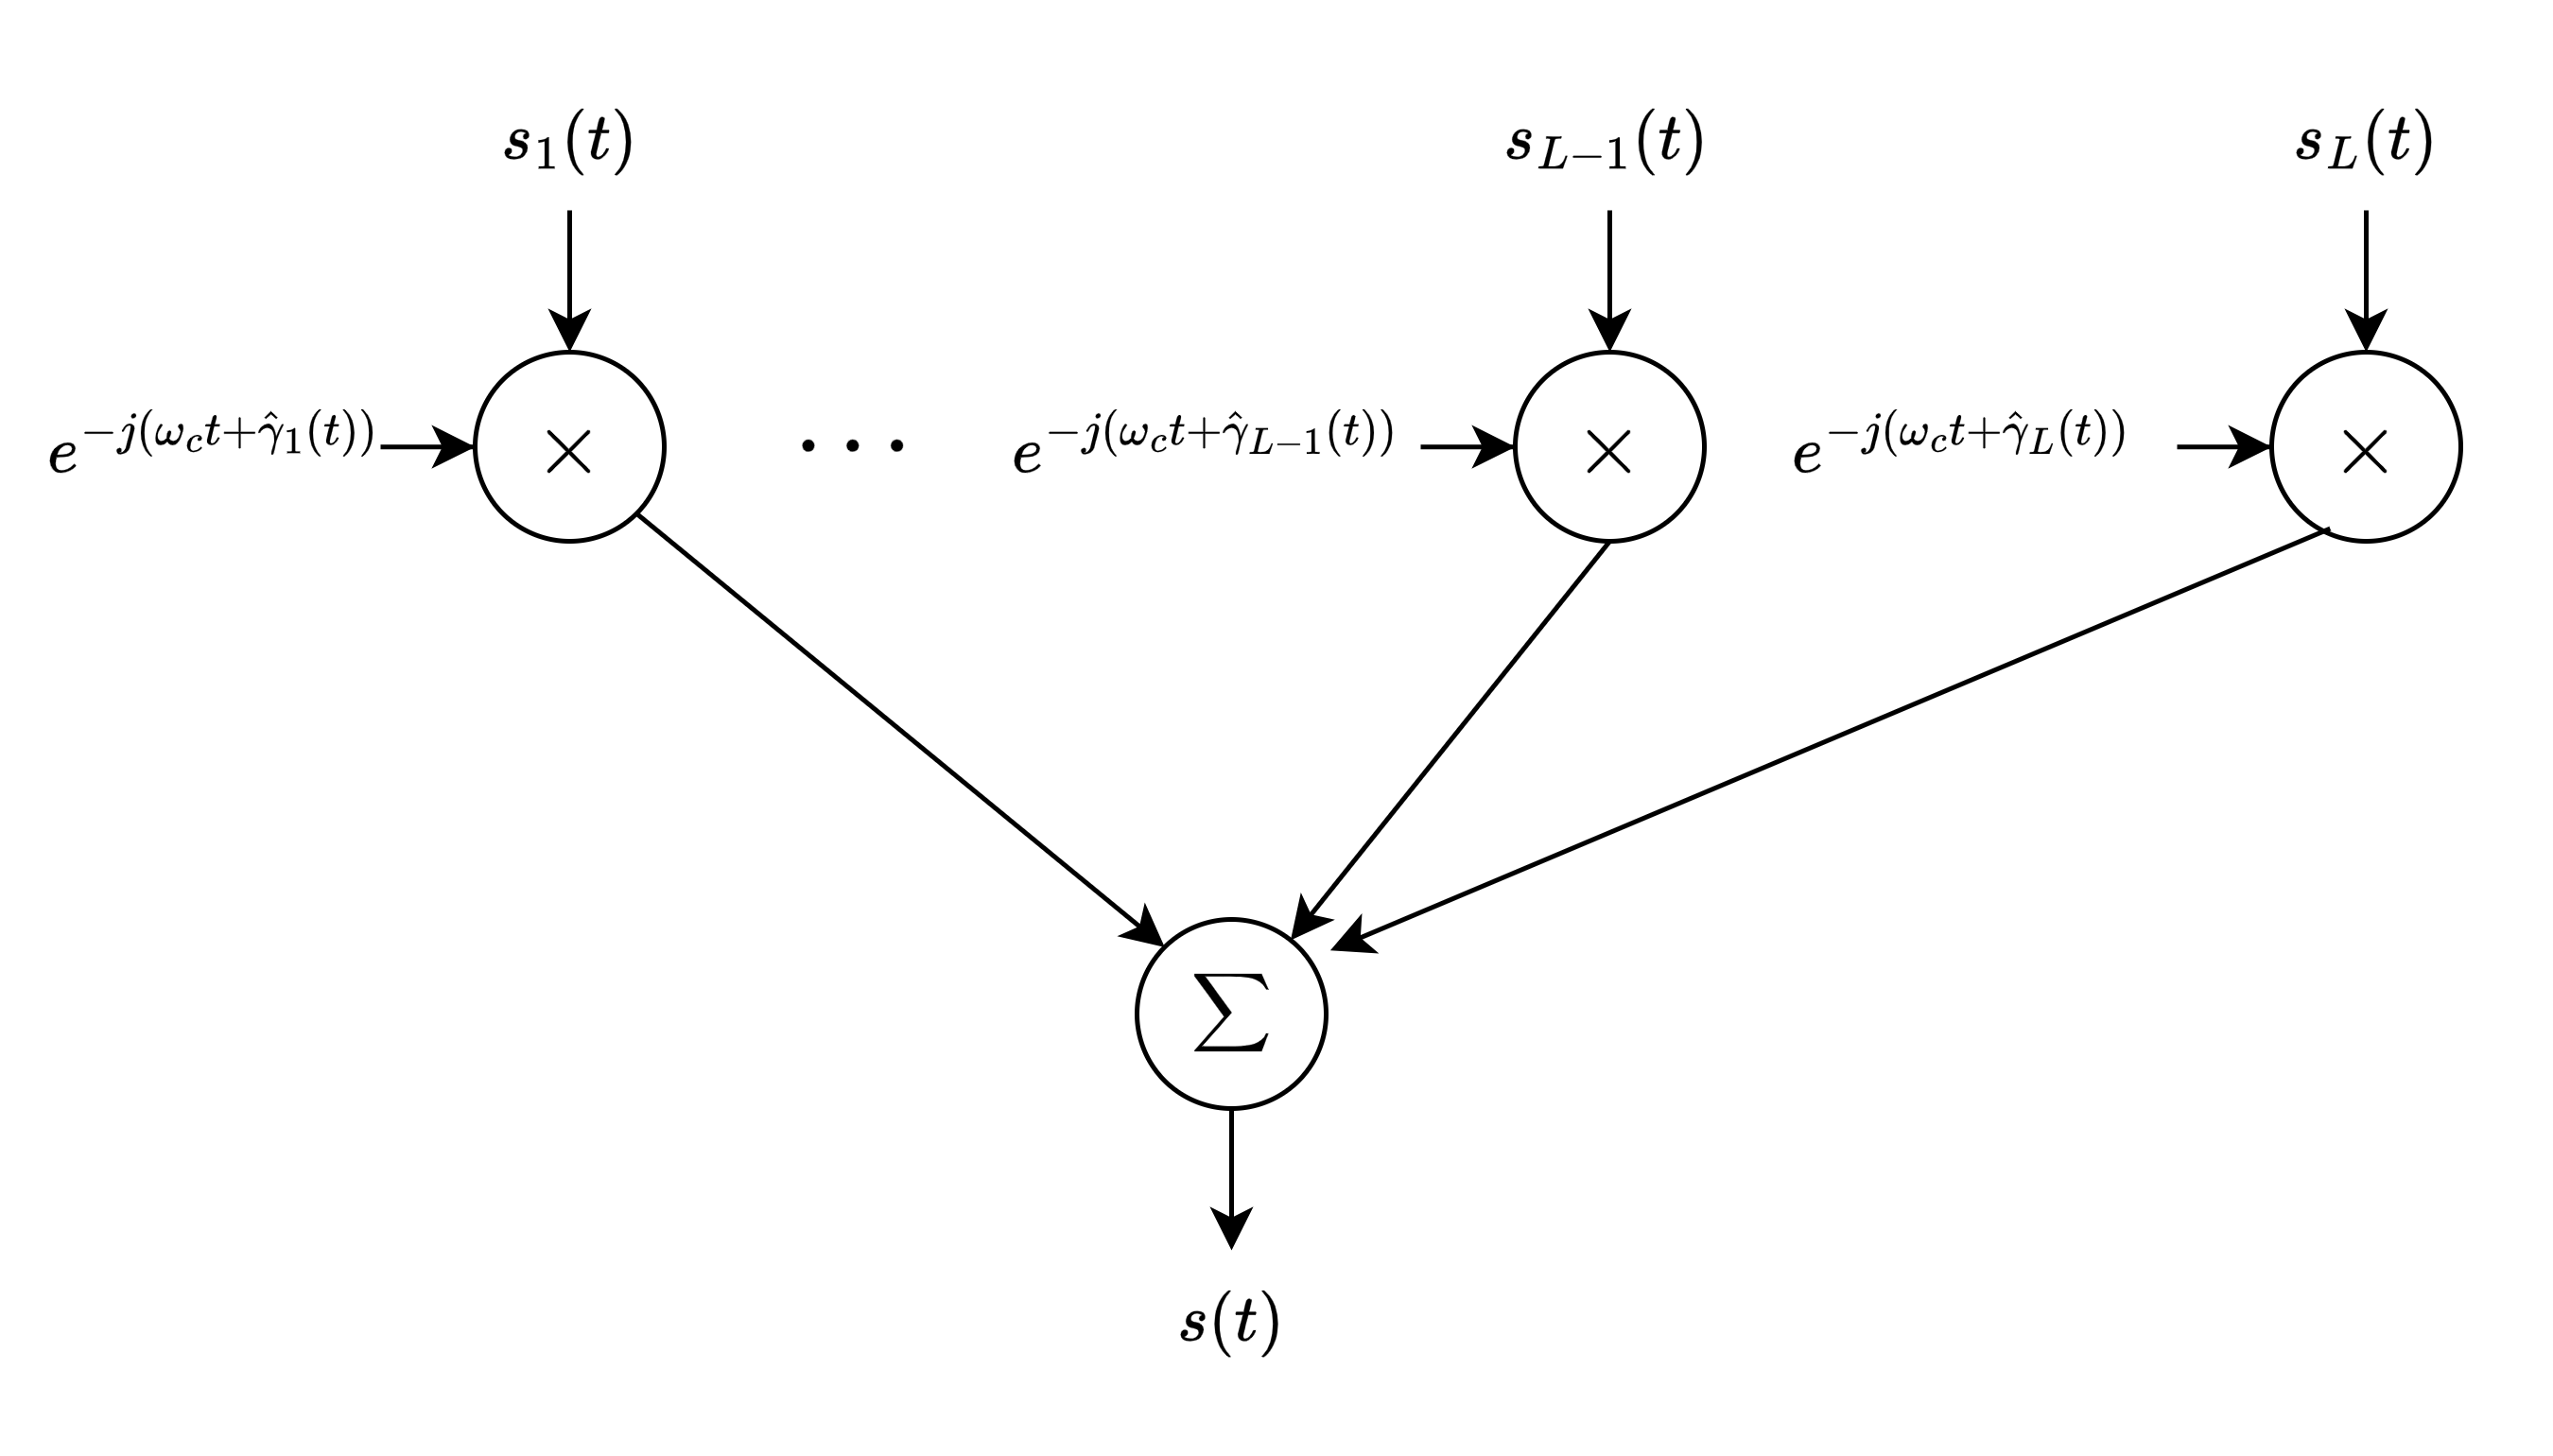
\includegraphics[width=0.6\textwidth]{egc.png}}}
			\caption{Equal Gain Combining}
			\label{fig::equal_gain_combining}
		\end{figure}
		
		The resulting phase error in each branch is denoted as
		
		$\varphi_i(t) = \gamma_i(t) - \hat{\gamma}_i(t)$
		
		The signal at the equal gain combiner output will then be
		
		\begin{equation*}
			s(t) = \sum_{i=1}^{M}{\left(r_i(t)e^{j(\phi(t) + \varphi_i(t))}+n_i(t)\right)} = e^{j\phi(t)}\sum_{i=1}^{M}{r_i(t)e^{j\varphi_i(t)}} + n(t)
		\end{equation*}
		
		If the noise on each branch $n_i(t)$ is independent and has noise PSD $N_0$. Then, the noise at the combiner output $n(t)$ has noise PSD $MN_0$.
		
		The corresponding observation vector is defined by
		
		\begin{equation*}
			\mathbf{r} = \begin{bmatrix}
				r_I \\
				r_Q
			\end{bmatrix}
		\end{equation*}
		
		where
		
		\begin{equation*}
			r_I = \sum_{i=1}^{M}{r_i\cos(\phi + \varphi_i)} + n_I
		\end{equation*}
		
		\begin{equation*}
			r_Q = \sum_{i=1}^{M}{r_i\sin(\phi + \varphi_i)} + n_Q
		\end{equation*}
		
		where $n_I$ and $n_Q$ are i.i.d. Gaussian Random variables with variance $M\sigma^2$
		
		First, we consider BPSK modulation. The probability of error should be the same for all symbols, so we consider $\phi = 0$. For given choices of $r_i$ and $\varphi_i$, we find that the probability of bit error is
		
		\begin{equation*}
			P_b = Q\left(\frac{\sum_{i=1}^{M}{r_i\cos(\varphi_i)}}{\sigma\sqrt{M}}\right)
		\end{equation*}
		 
		To find the average probability of bit error we have to integrate across the distributions for $\mathbf{r} = (r_1,...,r_M)$ and $\boldsymbol{\varphi} = (\varphi_1,...,\varphi_M)$.
		
		\begin{equation*}
			\bar{P}_b = \int_{\mathbf{r}}{\int_{\boldsymbol{\varphi}}{P_b(\mathbf{r},\boldsymbol{\varphi})p_{\boldsymbol{\varphi}}(\boldsymbol{\varphi})p_{\mathbf{R}}(\mathbf{r})d\boldsymbol{\varphi}}d\mathbf{r}}
		\end{equation*}
		
		\begin{equation*}
			= \int_{\mathbf{r}}{\int_{\boldsymbol{\varphi}}{Q\left(\frac{\sum_{i=1}^{M}{r_i\cos(\varphi_i)}}{\sigma\sqrt{M}}\right)p_{\boldsymbol{\varphi}}(\boldsymbol{\varphi})p_{\mathbf{R}}(\mathbf{r})d\boldsymbol{\varphi}}d\mathbf{r}}
		\end{equation*}
		
		If the elements $\mathbf{r}$ are independent then
		
		\begin{equation*}
			p_\mathbf{R}(\mathbf{r}) = \prod_{i=1}^{M}{p_{R_i}(r_i)} = \prod_{i=1}^{M}\left[\frac{\alpha_i\mu_i^{\mu_i}r_i^{\alpha_i\mu_i-1}}{\hat{r}_i^{\alpha_i\mu_i}\Gamma(\mu_i)}\text{exp}\left(\mu_i\frac{r_i^{\alpha_i}}{\hat{r}_i^{\alpha_i}}\right)\right]
		\end{equation*}
		
		Similarly, if the elements of $\boldsymbol{\varphi}$ are independent then
		
		\begin{equation*}
			p_{\boldsymbol{\varphi}}(\boldsymbol{\varphi}) = \prod_{i=1}^{M}{p_{\phi}(\phi)} = \prod_{i=1}^{M}\left[\frac{1}{2\pi}\frac{\text{exp}(\zeta_i\text{cos}(\varphi_i))}{I_0(\zeta_i)}\right], \quad -\pi < \varphi_i \leq \pi
		\end{equation*}
		
		The EGC output with phase error in the receiver branches can be written as:
		
		\begin{equation*}
			r = \sum_{i=1}^{M}{r_ie^{j\varphi_i}}/\sqrt{M}
		\end{equation*}
		 
		\item[3.] Let us now consider the time-invariant frequency-selective block-fading channel with 32 subchannels of bandwidth 2 MHz, with frequency response amplitudes being $1$ for odd subchannels and $\sqrt{2}$ for even subchannels, respectively. For the transmit power 10 mW and noise power-spectral density of $N_0=10^{-9}$ W/Hz determine the OFDM channel capacity. What is corresponding optimum power allocation strategy based on OFDM to achieve this channel capacity? Provide the corresponding OFDM transmitter and receiver configurations.
		
		\begin{equation*}
			C = \underset{P_i \ :\ \sum_i{P_i \leq P}}{\sum}{W\text{log}_2\left(1 + \frac{|H_i|^2P_i}{N_0W}\right)}
		\end{equation*}
		
		\begin{equation*}
			\frac{P_i}{P} = \begin{cases}
				\frac{1}{\rho_{tsh}} - \frac{1}{\rho_i} & \rho_i \geq \rho_{tsh} \\
				0 & \rho_i < \rho_{tsh}
			\end{cases}
		\end{equation*}
		
		where
		
		\begin{equation*}
			\rho_i = \frac{|H_i|^2P}{N_0W} = |H_i|^2\rho_0 
		\end{equation*}
		
		\begin{equation*}
			\rho_0 = \frac{P}{N_0W} = \frac{10 \times 10^{-3}}{10^{-9}(2 \times 10^6)} = 5
		\end{equation*}
		
		\begin{equation*}
			\rho_{\text{odd}} = |H_{\text{odd}}|^2\rho_0 = 5
		\end{equation*}
		
		\begin{equation*}
			\rho_{\text{even}} = |H_{\text{even}}|^2\rho_0 = 10
		\end{equation*}
		
		Assume $p_i \geq \rho_{tsh}\ \forall\ i$
		
		\begin{equation*}
			\sum_i{\frac{P_i}{P}} = 1
		\end{equation*}
		
		\begin{equation*}
			\Rightarrow \sum_i{\left(\frac{1}{\rho_{tsh}} - \frac{1}{\rho_i}\right)} = 1
		\end{equation*}
		
		\begin{equation*}
			\Rightarrow \frac{32}{\rho_{tsh}} - \frac{16}{\rho_{\text{odd}}} - \frac{16}{\rho_{\text{even}}} = 1
		\end{equation*}
		
		\begin{equation*}
			\Rightarrow \frac{32}{\rho_{tsh}} = 1 + \frac{16}{\rho_{\text{odd}}} + \frac{16}{\rho_{\text{even}}}
		\end{equation*}
		
		\begin{equation*}
			\Rightarrow \frac{32}{\rho_{tsh}} = 1 + \frac{16}{5} + \frac{16}{10} = 5.8
		\end{equation*}
		
		\begin{equation*}
			\Rightarrow \rho_{tsh} = \frac{32}{5.8} \approx 5.5172
		\end{equation*}
		
		Note that this is inconsistent with the assumption that $p_i \geq \rho_{tsh}\ \forall\ i$. Therefore, $\rho_{\text{odd}} < \rho_{tsh} \leq \rho_{\text{even}}$.
		
		\begin{equation*}
			\Rightarrow \sum_{i\ \text{even}}{\left(\frac{1}{\rho_{tsh}} - \frac{1}{\rho_i}\right)} = 1
		\end{equation*}
		
		\begin{equation*}
			\Rightarrow \frac{16}{\rho_{tsh}} - \frac{16}{\rho_{\text{even}}} = 1
		\end{equation*}
		
		\begin{equation*}
			\Rightarrow \frac{16}{\rho_{tsh}} = 1 + \frac{16}{\rho_{\text{even}}} = 1 + \frac{16}{10} = 2.6
		\end{equation*}
		
		\begin{equation*}
			\Rightarrow \rho_{tsh} = \frac{16}{2.6} \approx 6.1538
		\end{equation*}
		
		\begin{equation*}
			\therefore C = \sum_i{W\text{log}_2\left(1 + \frac{|H_i|^2P_i}{N_0W}\right)} = \sum_{i\ \text{even}}{W\text{log}_2\left[1 + \frac{|H_i|^2P}{N_0W}\left(\frac{P_i}{P}\right)\right]}
		\end{equation*}
		
		\begin{equation*}
			= \sum{W\text{log}_2\left[1 + \rho_{\text{even}}\left(\frac{P_\text{even}}{P}\right)\right]}
		\end{equation*}
		
		\begin{equation*}
			 = \sum{W\text{log}_2\left[1 + \rho_{\text{even}}\left(\frac{1}{\rho_{tsh}} - \frac{1}{\rho_{\text{even}}}\right)\right]}
		\end{equation*}
		
		\begin{equation*}
			 = \sum{W\text{log}_2\left(\frac{\rho_{\text{even}}}{\rho_{tsh}}\right)} = 16W\text{log}_2\left(\frac{\rho_{\text{even}}}{\rho_{tsh}}\right) \approx 22.4141\ \text{Mbps}
		\end{equation*}
		
		The optimum power allocation strategy is water filling.
		
		\begin{equation*}
			\frac{P_i}{P} = \begin{cases}
				\frac{1}{\rho_{tsh}} - \frac{1}{\rho_i} & \rho_i \geq \rho_{tsh} \\
				0 & \rho_i < \rho_{tsh}
			\end{cases}
		\end{equation*}
		
		\begin{equation*}
			\Rightarrow P_{\text{odd}} = 0\ \text{mW}
		\end{equation*}
		
		\begin{equation*}
			\Rightarrow P_{\text{even}} = P\left(\frac{1}{\rho_{tsh}} - \frac{1}{\rho_{\text{even}}}\right) = 10\left(\frac{1}{6.1538} - \frac{1}{10}\right) = 0.625\ \text{mW}
		\end{equation*}		
		
		\item[4.] This problem is related to MIMO wireless communications. Let $\mathbf{x}$ be transmitted vector, $\mathbf{y}$ be received vector, and $\mathbf{z}$ be (AWGN) noise vector, which are related by: $\mathbf{y}=\mathbf{Hx} + \mathbf{z}$, where $\mathbf{H}$ is the channel matrix. Determine the estimate of $\mathbf{x}$ to minimize the MSE. What is the minimum variance of error of this detector?
		
		\pagebreak
		We can use a Linear MMSE receiver to estimate of $\mathbf{x}$, which we denote as $\mathbf{\hat{x}}$. In this receiver, we chose a linear transformation matrix $\mathbf{A}$ to minimize the following MSE:
		
		$\text{MSE}(\mathbf{A}) = \langle \norm{\mathbf{\hat{x}} - \mathbf{x}}^2_F \rangle = \langle \norm{\mathbf{Ay} - \mathbf{x}}^2_F \rangle = \langle \norm{\mathbf{A}(\mathbf{Hx} + \mathbf{z}) - \mathbf{x}}^2_F \rangle$
		
		$ = \langle \norm{\mathbf{AHx} + \mathbf{Az} - \mathbf{x}}^2_F \rangle = \langle \norm{(\mathbf{AH} - \mathbf{I_{M_{Tx}}})\mathbf{x} + \mathbf{Az}}^2_F \rangle$
		
		$\norm{\mathbf{A}}_F$ is the Frobenius norm of a matrix and is defined as follows:
		
		$\norm{\mathbf{A}}_F = \sqrt{\text{Tr}(\mathbf{AA^{\dagger}})}$
		
		$\Rightarrow \text{MSE}(\mathbf{A}) = \langle \text{Tr}[((\mathbf{AH} - \mathbf{I_{M_{Tx}}})\mathbf{x} + \mathbf{Az})((\mathbf{AH} - \mathbf{I_{M_{Tx}}})\mathbf{x} + \mathbf{Az})^{\dagger}]\rangle$
		
		$ = \langle \text{Tr}[(\mathbf{AH} - \mathbf{I_{M_{Tx}}})\mathbf{xx^{\dagger}}(\mathbf{AH} - \mathbf{I_{M_{Tx}}})^{\dagger}] \rangle + \langle \text{Tr}[\mathbf{Azx^{\dagger}}(A\mathbf{H} - \mathbf{I_{M_{Tx}}})^{\dagger}] \rangle$
		
		$ + \langle \text{Tr}[(A\mathbf{H} - \mathbf{I_{M_{Tx}}})\mathbf{xz^{\dagger}A^{\dagger}}] \rangle + \langle \text{Tr}[\mathbf{Azz^{\dagger}A^{\dagger}}] \rangle$
		
		Assume that $\mathbf{x}$ and $\mathbf{z}$ are independent and the elements of $\mathbf{x}$ and $\mathbf{z}$ are zero-mean i.i.d. random variables.
		
		$\Rightarrow \text{MSE}(\mathbf{A}) = \text{Tr}[\rho(\mathbf{AH} - \mathbf{I_{M_{Tx}}})(\mathbf{AH} - \mathbf{I_{M_{Tx}}})^{\dagger}] + \text{Tr}[N_0\mathbf{AA^{\dagger}}]$
		
		$ = \text{Tr}[\rho(\mathbf{AH} - \mathbf{I_{M_{Tx}}})(\mathbf{AH} - \mathbf{I_{M_{Tx}}})^{\dagger} + N_0\mathbf{AA^{\dagger}}]$
		
		We can minimize the MSE w.r.t $\mathbf{A}$ by setting the MSE variation w.r.t $\mathbf{A}$ to zero.
		
		$\delta(\text{MSE}) = \text{Tr}\left\{\delta\mathbf{A}[\rho\mathbf{H}(\mathbf{AH} - \mathbf{I_{M_{Tx}}})^{\dagger} + N_0\mathbf{A}^{\dagger}]\right.$
		
		$ \left. + [\rho(\mathbf{AH} - \mathbf{I_{M_{Tx}}})\mathbf{H}^{\dagger} + N_0\mathbf{A}]\delta\mathbf{A}^{\dagger}\right\} = 0$
		
		We can then solve for $\mathbf{A}$. Doing so results in the following:
		
		$\mathbf{A_{MMSE}} = \mathbf{H^{\dagger}}(\mathbf{HH^{\dagger}} + \mathbf{I_{M_{Rx}}}/\text{SNR})^{-1} = (\mathbf{H^{\dagger}H} + \mathbf{I_{M_{Tx}}}/\text{SNR})^{-1}\mathbf{H^{\dagger}}$
		
		where $SNR = \rho/N_0$
		
		The transmitted vector can be estimated from the receiver vector as follows:
		
		$\mathbf{\hat{x}} = \mathbf{A_{MMSE}y} =(\mathbf{H^{\dagger}H} + \mathbf{I_{M_{Tx}}}/\text{SNR})^{-1}\mathbf{H^{\dagger}y}$
		
		The minimum variance of error will be:
		
		$\text{Var}\{(\mathbf{Az},\mathbf{d})\} = N_0\norm{\mathbf{A^{\dagger}d}}^2$
		
		where $\mathbf{d} = \mathbf{x} - \mathbf{\hat{x}}$
		
		\item[5.] The space-time code for number of transmit antennas $M_{TX}=4$, number of receive antennas $M_{RX}=1$, and number of channel's uses $N=4$ is described by the following signaling matrix:
		
		\begin{equationCenter}
			\mathbf{X} = \begin{bmatrix}
				x_1 & -x_2^* & -x_3^* &  0 \\ 
				x_2 &  x_1^* &  0     &  x_3^* \\
				x_3 &  0     &  x_1^* & -x_2^* \\
				0   & -x_3^* &  x_2^* &  x_1^*
			\end{bmatrix}
		\end{equationCenter}
		
		\begin{enumerate}
			\item Can this space-time block code be used to design the receiver that will result in spatial interference cancellation? If so describe the corresponding receiver configuration. What is the code rate of this space-time code?
			
			\begin{equation*}
				\mathbf{Y} = \mathbf{H}\mathbf{X} + \mathbf{Z}
			\end{equation*}
			
			\begin{equation*}
				\begin{bmatrix}
					y_1 \\ y_2 \\ y_3 \\ y_4
				\end{bmatrix}^T = \begin{bmatrix}
					h_1 & h_2 & h_3 & h_4
				\end{bmatrix}\begin{bmatrix}
					x_1 & -x_2^* & -x_3^* &  0 \\ 
					x_2 &  x_1^* &  0     &  x_3^* \\
					x_3 &  0     &  x_1^* & -x_2^* \\
					0   & -x_3^* &  x_2^* &  x_1^*
				\end{bmatrix} + \begin{bmatrix}
					z_1 \\ z_2 \\ z_3 \\ z_4
				\end{bmatrix}^T
			\end{equation*}
			
			\begin{equation*}
				\begin{bmatrix}
					y_1 \\ y_2 \\ y_3 \\ y_4
				\end{bmatrix} = \begin{bmatrix}
					 h_1x_1   + h_2x_2   + h_3x_3 \\
					-h_1x_2^* + h_2x_1^* - h_4x_3^* \\
					-h_1x_3^* + h_3x_1^* + h_4x_2^* \\
					 h_2x_3^* - h_3x_2^* + h_4x_1^*
				\end{bmatrix} + \begin{bmatrix}
					z_1 \\ z_2 \\ z_3 \\ z_4
				\end{bmatrix}
			\end{equation*}
			
			\begin{equation*}
				\begin{bmatrix}
					y_1 \\ y_2^* \\ y_3^* \\ y_4^*
				\end{bmatrix} = \begin{bmatrix}
					 h_1x_1   + h_2x_2   + h_3x_3 \\
					-h_1^*x_2 + h_2^*x_1 - h_4^*x_3 \\
					-h_1^*x_3 + h_3^*x_1 + h_4^*x_2 \\
					 h_2^*x_3 - h_3^*x_2 + h_4^*x_1
				\end{bmatrix} + \begin{bmatrix}
					z_1 \\ z_2^* \\ z_3^* \\ z_4^*
				\end{bmatrix}
			\end{equation*}
			
			\begin{equation*}
				\begin{bmatrix}
					y_1 \\ y_2^* \\ y_3^* \\ y_4^*
				\end{bmatrix} = \begin{bmatrix}
					h_1   &  h_2   &  h_3 \\
				    h_2^* & -h_1^* & -h_4^* \\
					h_3^* &  h_4^* & -h_1^* \\
					h_4^* & -h_3^* &  h_2^*
				\end{bmatrix} \begin{bmatrix}
					x_1 \\ x_2 \\ x_3
				\end{bmatrix} + \begin{bmatrix}
					z_1 \\ z_2^* \\ z_3^* \\ z_4^*
				\end{bmatrix}
			\end{equation*}
			
			\begin{equation*}
				\mathbf{\tilde{Y}} = \mathbf{\tilde{H}x} + \mathbf{\tilde{z}}
			\end{equation*}
			
			\begin{equation*}
				\mathbf{\tilde{H}^\dagger\tilde{Y}} = \mathbf{\tilde{H}^\dagger\tilde{H}x} + \mathbf{\tilde{H}^\dagger\tilde{z}}
			\end{equation*}
			
			\begin{equation*}
				\mathbf{\tilde{H}^\dagger\tilde{H}} = \begin{bmatrix}
					h_1^* &  h_2 &  h_3 &  h_4 \\
					h_2^* & -h_1 &  h_4 & -h_3 \\
					h_3^* & -h_4 & -h_1 &  h_2
				\end{bmatrix} \begin{bmatrix}
					h_1   &  h_2   &  h_3 \\
				    h_2^* & -h_1^* & -h_4^* \\
					h_3^* &  h_4^* & -h_1^* \\
					h_4^* & -h_3^* &  h_2^*
				\end{bmatrix}
			\end{equation*}
			
			\begin{equation*}
				= \begin{bmatrix}
					|h_1|^2 + \cdots + |h_4|^2 & h_3h_4^* - h_3^*h_4 & h_2^*h_4 - h_2h_4^* \\
					h_3^*h_4 - h_3h_4^* & |h_1|^2 + \cdots + |h_4|^2 & h_1h_4^* - h_1^*h_4 \\
					h_2h_4^* - h_2^*h_4 & h_1^*h_4 - h_1h_4^* & |h_1|^2 + \cdots + |h_4|^2
				\end{bmatrix}
			\end{equation*}
			
			Note that there are multiple terms of the form:
			
			\begin{equation*}
				a - a^* = \text{Re}\{a\} + j\text{Im}\{a\} - (\text{Re}\{a\} - j\text{Im}\{a\}) = j2\text{Im}\{a\}
			\end{equation*}
			
			For the space-time block code to result in spatial interference cancellation, we must be able to write $\mathbf{\tilde{H}^{\dagger}\tilde{H}}$ as $\alpha\mathbf{I}$.
			
			Note that this is not the case in general for the code provided, so it does \textbf{\underline{not}} result in spatial interference cancellation.
			
			However, in a real orthogonal design, the matrix $\mathbf{\tilde{H}}$ is real. This results in $\mathbf{\tilde{H}^\dagger\tilde{H}} = (|h_1|^2 + \cdots + |h_4|^2)\mathbf{I}$. In other words, spatial interference cancellation is realized.
			
			In this case, the coding rate would be $3/4$, because 3 symbols are transmitted in 4 symbol intervals.
			
			\item Represent the signaling matrix $\mathbf{X}$ in the same fashion as for linear space-time (LST) codes. If the channel matrix is given by $\mathbf{H}=\begin{bmatrix} h_1 & h_2 & h_3 & h_4 \end{bmatrix}$ using detection approach for LST determine the equations for the estimated symbols $\hat{x}_i$.
			
			Let $x_1 = a_1 + jb_1$, $x_2 = a_2 + jb_2$, and $x_3 = a_3 + jb_3$.
			
			\begin{equation*}
				\mathbf{X} = a_1\mathbf{A_1} + jb_1\mathbf{B_1} + \cdots + a_3\mathbf{A_3} + jb_3\mathbf{B_3}
			\end{equation*}
			
			\begin{equation*}
				= a_1\begin{bmatrix}
					1 & 0 & 0 & 0 \\
					0 & 1 & 0 & 0 \\
					0 & 0 & 1 & 0 \\
					0 & 0 & 0 & 1
				\end{bmatrix} + jb_1\begin{bmatrix}
					1 &  0 &  0 &  0 \\
					0 & -1 &  0 &  0 \\
					0 &  0 & -1 &  0 \\
					0 &  0 &  0 & -1
				\end{bmatrix}
			\end{equation*}
			
			\begin{equation*}
				 + a_2\begin{bmatrix}
					0 & -1 & 0 &  0 \\
					1 &  0 & 0 &  0 \\
					0 &  0 & 0 & -1 \\
					0 &  0 & 1 &  0
				\end{bmatrix} + jb_2\begin{bmatrix}
					0 & 1 &  0 & 0 \\
					1 & 0 &  0 & 0 \\
					0 & 0 &  0 & 1 \\
					0 & 0 & -1 & 0
				\end{bmatrix}
			\end{equation*}
			
			\begin{equation*}
				+ a_3\begin{bmatrix}
					0 &  0 & -1 & 0 \\
					0 &  0 &  0 & 1 \\
					1 &  0 &  0 & 0 \\
					0 & -1 &  0 & 0
				\end{bmatrix} + jb_3\begin{bmatrix}
					0 & 0 & 1 &  0 \\
					0 & 0 & 0 & -1 \\
					1 & 0 & 0 &  0 \\
					0 & 1 & 0 &  0
				\end{bmatrix}
			\end{equation*}
			
			We can define define the transmitted vector as follows:
			
			\begin{equation*}
				\mathbf{\tilde{x}} = \begin{bmatrix}
					a_1 & b_1 & \cdots & a_3 & b_3
				\end{bmatrix}^T
			\end{equation*}
			
			We can also define the noise vector as $\mathbf{\tilde{z}} = \text{vec}(\mathbf{Z})$ and the received vector as $\mathbf{\tilde{y}} = \text{vec}(\mathbf{Y})$.
			
			Next, if we define the modified channel matrix as
			
			\begin{equation*}
				\mathbf{\tilde{H}} = \begin{bmatrix}
					\text{vec}(\mathbf{HA_1}) & \text{vec}(j\mathbf{HB_1}) & \cdots & \text{vec}(\mathbf{HA_3}) & \text{vec}(j\mathbf{HB_3})
				\end{bmatrix}
			\end{equation*} 
			
			\begin{equation*}
				\mathbf{HA_1} = \begin{bmatrix}
					h_1 & h_2 & h_3 & h_4
				\end{bmatrix}\begin{bmatrix}
					1 & 0 & 0 & 0 \\
					0 & 1 & 0 & 0 \\
					0 & 0 & 1 & 0 \\
					0 & 0 & 0 & 1
				\end{bmatrix}
			\end{equation*}
			
			\begin{equation*}
				= \begin{bmatrix}
					h_1 & h_2 & h_3 & h_4
				\end{bmatrix}
			\end{equation*}
			
			\begin{equation*}
				\mathbf{HB_1} = \begin{bmatrix}
					h_1 & h_2 & h_3 & h_4
				\end{bmatrix}\begin{bmatrix}
					1 &  0 &  0 &  0 \\
					0 & -1 &  0 &  0 \\
					0 &  0 & -1 &  0 \\
					0 &  0 &  0 & -1
				\end{bmatrix}
			\end{equation*}
			
			\begin{equation*}
				 = \begin{bmatrix}
					h_1 & -h_2 & -h_3 & -h_4
				\end{bmatrix}
			\end{equation*}
			
			\begin{equation*}
				\mathbf{HA_2} = \begin{bmatrix}
					h_1 & h_2 & h_3 & h_4
				\end{bmatrix}\begin{bmatrix}
					0 & -1 & 0 &  0 \\
					1 &  0 & 0 &  0 \\
					0 &  0 & 0 & -1 \\
					0 &  0 & 1 &  0
				\end{bmatrix}
			\end{equation*}
			
			\begin{equation*}
				= \begin{bmatrix}
					h_2 & -h_1 & h_4 & -h_3
				\end{bmatrix}
			\end{equation*}
			
			\begin{equation*}
				\mathbf{HB_2} = \begin{bmatrix}
					h_1 & h_2 & h_3 & h_4
				\end{bmatrix}\begin{bmatrix}
					0 & 1 &  0 & 0 \\
					1 & 0 &  0 & 0 \\
					0 & 0 &  0 & 1 \\
					0 & 0 & -1 & 0
				\end{bmatrix}
			\end{equation*}
			
			\begin{equation*}
				= \begin{bmatrix}
					h_2 & h_1 & -h_4 & h_3
				\end{bmatrix}
			\end{equation*}
			
			\begin{equation*}
				\mathbf{HA_3} = \begin{bmatrix}
					h_1 & h_2 & h_3 & h_4
				\end{bmatrix}\begin{bmatrix}
					0 &  0 & -1 & 0 \\
					0 &  0 &  0 & 1 \\
					1 &  0 &  0 & 0 \\
					0 & -1 &  0 & 0
				\end{bmatrix}
			\end{equation*}
			
			\begin{equation*}
				= \begin{bmatrix}
					h_3 & -h_4 & -h_1 & h_2
				\end{bmatrix}
			\end{equation*}
			
			\begin{equation*}
				\mathbf{HB_3} = \begin{bmatrix}
					h_1 & h_2 & h_3 & h_4
				\end{bmatrix}\begin{bmatrix}
					0 & 0 & 1 &  0 \\
					0 & 0 & 0 & -1 \\
					1 & 0 & 0 &  0 \\
					0 & 1 & 0 &  0
				\end{bmatrix}
			\end{equation*}
			
			\begin{equation*}
				= \begin{bmatrix}
					h_3 & h_4 & h_1 & -h_2
				\end{bmatrix}
			\end{equation*}
			
			\begin{equation*}
				\Rightarrow \mathbf{\tilde{H}} = \begin{bmatrix}
					h_1 &  jh_1 &  h_2 &  jh_2 &  h_3 &  jh_3 \\
					h_2 & -jh_2 & -h_1 &  jh_1 & -h_4 &  jh_4 \\
					h_3 & -jh_3 &  h_4 & -jh_4 & -h_1 &  jh_1 \\
					h_4 & -jh_4 & -h_3 &  jh_3 &  h_2 & -jh_2
				\end{bmatrix}
			\end{equation*}
			
			We can then use QR decomposition to write $\mathbf{\tilde{H}}$ as follows:
			
			\begin{equation*}
				\mathbf{\tilde{H}} = \mathbf{\tilde{Q}}\mathbf{\tilde{R}}
			\end{equation*}
		\end{enumerate}
		
		where $\mathbf{\tilde{Q}}$ is a unitary matrix and $\mathbf{\tilde{R}}$ is an upper triangular matrix.
		
		Next, we can express the received vector $\mathbf{\tilde{y}}$ as follows:
		
		\begin{equation*}
			\mathbf{\tilde{y}} = \mathbf{\tilde{H}\tilde{x}} + \mathbf{\tilde{z}} = \mathbf{\tilde{Q}\tilde{R}\tilde{x}} + \mathbf{\tilde{z}}
		\end{equation*}
		
		\begin{equation*}
			\Rightarrow \mathbf{\tilde{Q}^{\dagger}\tilde{y}} = \mathbf{\tilde{R}\tilde{x}} + \mathbf{\tilde{Q}^{\dagger}\tilde{z}}
		\end{equation*}
		
		We can find $\mathbf{\tilde{x}}$ by minimizing the error between $\mathbf{\tilde{R}\tilde{x}}$ and $\mathbf{\tilde{Q}^{\dagger}\tilde{y}}$.
		
		\begin{equation*}
			\mathbf{\hat{x}} = \underset{\mathbf{\tilde{x}}}{\text{arg min}}{\norm{\mathbf{\tilde{Q}^{\dagger}\tilde{y}} - \tilde{R}\tilde{x}}_F}
		\end{equation*}
		
		Finally, we can get $\hat{x}_i$ from $\mathbf{\hat{x}}$ as follows:
		
		\begin{equation*}
			\mathbf{\hat{x}} = \begin{bmatrix}\text{Re}(\hat{x}_1) & \text{Im}(\hat{x}_1) & \cdots & \text{Re}(\hat{x}_3) & \text{Im}(\hat{x}_3)\end{bmatrix}^T
		\end{equation*}
		
		
	\end{enumerate}
\end{document}